\lab{Geometric Optics}\label{lab:geometric-optics}

\apparatus
\equipn{optical bench}{1/group}
\equip{converging lens, $f=50$ cm, 5 cm diam}{1/group}
\equipn{converging lens, $f=5$ cm}{1/group}
\equipn{lamp and arrow-shaped mask}{1/group}
\equipn{frosted glass screen}{1/group}

\begin{goals}

\item[] Observe a real image formed by a convex lens, and
determine its focal length.

\item[] Construct a telescope and measure its angular magnification.
\end{goals}

\introduction

The credit for invention of the telescope is disputed, but
Galileo was probably the first person to use one for
astronomy. He first heard of the new invention when a
foreigner visited the court of his royal patrons and
attempted to sell it for an exorbitant price. Hearing
through second-hand reports that it consisted of two lenses,
Galileo sent an urgent message to his benefactors not to buy
it, and proceeded to reproduce the device himself. An early
advocate of simple scientific terminology, he wanted the
instrument to be called the ``occhialini,'' Italian for
``eye-thing,'' rather than the Greek ``telescope.''

His astronomical observations soon poked some gaping holes
in the accepted Aristotelian view of the heavens. Contrary
to Aristotle's assertion that the heavenly bodies were
perfect and without blemishes, he found that the moon had
mountains and the sun had spots (the marks on the moon
visible to the naked eye had been explained as optical
illusions or atmospheric phenomena). This put the heavens on
an equal footing with earthly objects, paving the way for
physical theories that would apply to the whole universe,
and specifically for Newton's law of gravity. He also
discovered the four largest moons of Jupiter, and demonstrated
his political savvy by naming them the ``Medicean satellites''
after the powerful Medici family. The fact that they
revolved around Jupiter rather than the earth helped make
more plausible Copernicus' theory that the planets did not
revolve around the earth but around the sun. Galileo's ideas
were considered subversive, and many people refused to look
through his telescope, either because they thought it was an
illusion or simply because it was supposed to show things
that were contrary to Aristotle.


\widefigcaption{op-geo-telescope}{A refracting telescope}\label{fig:telescope}

The figure on the next page
shows the simplest refracting telescope. The
object is assumed to be at infinity, so a real image is
formed at a distance from the objective lens equal to its
focal length, $f_o$. By setting up the eyepiece at a
distance from the image equal to its own focal length,
$f_E$, light rays that were parallel are again made parallel.

The point of the whole arrangement is angular magnification.
The small angle $\alpha_1$ is converted to a large
$\alpha_2$. It is the small angular size of distant objects
that makes them hard to see, not their distance. There is no
way to tell visually whether an object is a thirty meters
away or thirty billion. (For objects within a few meters,
your brain-eye system gives you a sense of depth based on
parallax.) The Pleiades star cluster can be seen more easily
across many light years than Mick Jagger's aging lips across
a stadium. People who say the flying saucer ``looked as big
as an aircraft carrier'' or that the moon ``looks as big as
a house'' don't know what they're talking about. The
telescope does not make things ``seem closer'' --- since the
rays coming at your eye are parallel, the final virtual
image you see is at infinity. The angular magnification is given by
\begin{equation*}
      M_A  =  \alpha_2/\alpha_1   
\end{equation*}
(to be measured directly in this lab)
\begin{equation*}
      M_A  =  f_o/f_E   
\end{equation*}
(theory).

\observations

\labpart{ Focal length of the lenses}
In this part of the lab, you'll accurately determine the focal lengths of the two
lenses being used for the telescope. They are poorly quality-controlled, and I've
found that the labeled values are off by as much as 10\%.

Start with the short-focal-length lens you're going to use as your eyepiece.
Use the lens to project a real image on the
frosted glass screen. For your object, use the lamp with the
arrow-shaped aperture in front of it. Make sure to lock down
the parts on the optical bench, or else they may tip over
and break the optics!

For the long-focal-length lens you're going to use as your objective, you will
probably be unable to do a similar determination on a one-meter optical bench.
Improvising a similar setup without the bench will still give you a much more
accurate value than the one written on the label.

A careful measurement here pays off later by making the focus in part B much
easier to find. This is especially true for the longer-focal-length lens.
To improve the quality of your result, do the kind of thing they do at the
optometrist --- ``which is better, 1 or 2?'' Have several people do independent
determinations of the best focus.

\labpart{ The telescope}

Use your optical bench and your two known lenses to build a
telescope.
 Since the telescope is a device for viewing objects
at infinity, you'll want to take it outside.

The best method for determining the angular magnification
is to observe the same object with both eyes open, with one
eye looking through the telescope and one seeing the object
without the telescope. Good precision can be obtained, for
example, by looking at a large object like a coke machine,
and determining that a small part of it, whose size you
can measure with a ruler, appears, when magnified, to cover some larger part
of it, which you can also measure. The figures on p.~\pageref{fig:telescope-terrier}
show a simulation of what the superimposed images should look like and of
how it would look if the telescope is not yet adjusted quite correctly.

Your brain is not capable of focusing one eye at one distance, and
the other at another distance. Therefore it's important to get your
telescope adjusted precisely so that the image is at infinity.
You can do this by focusing your naked eye on a distant object, and
then moving the objective until the image pops into focus in the
other eye. Theoretically this would be accomplished simply by setting
the lenses at the distance shown in the diagram, but in reality,
a small amount of further adjustment is necessary, because of the
uncertainty in the measured focal lengths.

A good quick test of the focus is to pick someone who's nearsighted
and see if they can focus on the image without their glasses on.
If they can, then the image is not at infinity, because nearsighted
people can't focus on an image that's at infinity.

\prelab

\prelabquestion    \emph{Skip this question if you were assigned problem
m4_ifdef([:__sn:],[:%
12-64 from Simple Nature,%
:])%
m4_ifdef([:__lm:],[:%
31-22 from Light and Matter,%
:])%
.} 
In part A, do you want the object to be closer to the
lens than the lens' focal length, exactly at a distance of
one focal length, or farther than the focal length?
What about the screen?

\prelabquestion  Plan what measurements you will make in part A and how
you will use them to determine the lenses' focal length.

\prelabquestion
It's disappointing to construct a telescope with
a very small magnification. Given a selection of lenses, plan
how you can make a telescope with the greatest possible
angular magnification.

\analysis

Determine the focal length of the two lenses, with error bars.

Find the angular magnification of your telescope from your
data, with error bars, and compare with theory. Do they
agree to within the accuracy of the measurement?
Give a probabilistic interpretation, as in the example
in appendix \ref{appendix:basicerranal}.
See the example at the end of appendix \ref{appendix:errpropagation} of how to
test for equality between two numbers that both have error bars.

\pagebreak

\begin{figure*}
  \includegraphics{../figs/op-geo-terrier}\label{fig:telescope-terrier}
\end{figure*}
